\chapter{认知时空几何学 — 块宇宙、切片演化与元动力学}

在前面章节确立认知空间流形结构后，这里需要明确一个建模问题：时间应被处理为流形演化的\textbf{外部参数}，还是流形自身的\textbf{内部维度}？
本章将物理时间 $t$（热力学流逝）与心理时间 $\tau$（逻辑序）严格解耦，给出\textbf{“切片演化”}与\textbf{“块宇宙”}两种对偶几何视角。
核心论点是：高阶智能可通过把外部时间内化为内部维度，在\textbf{$N+1$ 维超流形}上实现对历史表征与未来约束的统一操作，即\textbf{“元动力学 (Meta-Dynamics)”}。

\section{时间的双重性：参数 \texorpdfstring{$t$}{t} 与 维度 \texorpdfstring{$\tau$}{τ}}

由于智能系统并非单纯地栖居于物理时空之中，而是构建了一个独立的内蕴时空，为了精确描述这一机制，我们必须在数学上严格区分两种截然不同性质的“时间”。

\smalltitle{1. 物理时间 (\texorpdfstring{$t$}{t}, Process Time) —— 热力学的流逝}

\begin{itemize}
    \item \textbf{定义}：这是 \textbf{TDCI 循环} 的迭代步数，是微观层 ($L_{micro}$) 采样物理信号的频率，也是芯片时钟或神经脉冲的节律。
    \item \textbf{物理本质}：它是动力学方程中的 \textbf{演化参数 (Evolution Parameter)}，对应于偏微分方程中的 $\partial_t$。
    \item \textbf{热力学特征}：它是 \textbf{不可逆的 (Irreversible)}。它标记了系统熵增的方向，代表了“算力的消耗”与“寿命的流逝”。智能体无法在 $t$ 的轴线上后退，这是存在的代价。
\end{itemize}

\smalltitle{2. 心理时间 (\texorpdfstring{$\tau$}{τ}, Geometric Time) —— 几何的维度}

\begin{itemize}
    \item \textbf{定义}：这是 \textbf{底流形 $\mathcal{M}$} 上被“空间化”了的时间轴，是逻辑推理的序 (Order) 与因果链条的长度。
    \item \textbf{几何本质}：它是流形的一个 \textbf{坐标维度 (Coordinate Dimension)}，即 $x^0 = \tau$。
    \item \textbf{动力学特征}：它是 \textbf{可遍历的 (Traversable)}。智能体可以在 $\tau$ 轴上自由地进行“正向模拟（预测）”或“逆向搜索（回忆）”。在 $\tau$ 维度上的移动，消耗的是 $t$ 维度上的能量。
\end{itemize}

\begin{theorem}[维克转动假说 / Wick Rotation Hypothesis]
    高阶智能的涌现，源于系统通过 \textbf{维克转动 ($t \to i\tau$)}，将外部流逝的物理时间 $t$，卷曲、冻结为内部可操作的几何维度 $\tau$。
    $$ \mathcal{M}_{dynamic}^{(t)} \xrightarrow{\text{Internalization}} \mathcal{M}_{static}^{(\tau)} $$
\end{theorem}
这里“维克转动”是类比性的几何语言，用于表达“将时间内化为可操作维度”的机制，并不要求物理时间作真正的解析延拓。

\section{视角 I：切片演化观 — \texorpdfstring{$\mathcal{M}^{(N)}$}{M(N)} 随 \texorpdfstring{$t$}{t} 的流动}

这是低阶智能（如昆虫、基础控制系统）及微观层 ($L_{micro}$) 的典型图景。在该视角下，流形不显式包含时间维度，只描述当下空间结构。

\smalltitle{几何定义：瞬时切片 (Instantaneous Slice)}

\begin{itemize}
    \item \textbf{维度}：流形 $\mathcal{M}$ 是 $N$ 维的纯空间结构（仅包含语义关联，不包含因果历史）。
    \item \textbf{状态}：认知场是定义在切片上的瞬时快照 $\Psi(\mathbf{x}, t)$。
    \item \textbf{度量}：$g_{ij}(\mathbf{x}, t)$ 仅描述概念间的共现距离，不包含时序信息。
\end{itemize}

\smalltitle{动力学特征：哈密顿流 (Hamiltonian Flow)}

系统遵循 \textbf{柯西初值问题 (Cauchy Problem)}：给定 $t$ 时刻的状态，计算 $t+dt$ 时刻的状态。
$$ \frac{\partial \Psi}{\partial t} = \hat{H}(\mathbf{x}) \Psi $$
\begin{itemize}
    \item \textbf{无记忆性}：系统只受当前时刻的 \textbf{动量 (Momentum)} 和 \textbf{势能 (Potential)} 驱动。过去的历史仅以“当前的速度”形式存在，未来的目标仅以“当前的梯度”形式存在。
    \item \textbf{马尔可夫性质}：$P(S_{t+1} | S_t, S_{t-1}, \dots) = P(S_{t+1} | S_t)$。
\end{itemize}

\smalltitle{智能形态：当下的囚徒}

\begin{itemize}
    \item \textbf{优势}：\textbf{实时性}。计算量极小，无需维护庞大的历史数据，适合生存反射。
    \item \textbf{缺陷}：\textbf{时盲 (Time-Blindness)}。无法理解“跨时间”的因果关系，无法进行反事实推理（Counterfactual Reasoning）。
    \item \textbf{物种对应}：\textbf{Class I/II 智能}（如单细胞生物、无状态的 RNN）。它们活在永恒的“现在”。
\end{itemize}

\section{视角 II：块宇宙观 — \texorpdfstring{$\mathcal{M}^{(N+1)}$}{M(N+1)} 的静态晶体}

这是高阶智能（如人类、AGI）及宏观层 ($L_{macro}$) 的图景。在该视角下，时间被整合为空间的一部分，形成静态超流形。

\smalltitle{几何定义：超流形 (Hyper-Manifold)}

\begin{itemize}
    \item \textbf{维度}：流形 $\mathcal{M}$ 扩张为 $N+1$ 维，其中第 $0$ 维是心理时间 $\tau$。
    \item \textbf{度量结构}：为了在几何上区分“空间关联”与“时间因果”，流形必须拥有 \textbf{类闵可夫斯基度量 (Pseudo-Riemannian Metric)}：
    $$ ds^2 = -c_{cog}^2 d\tau^2 + g_{ij} dx^i dx^j $$
    \begin{itemize}
        \item \textbf{$c_{cog}$ (认知光速)}：定义了思维传播的因果视界。
        \item \textbf{类时区间 ($ds^2 < 0$)}：代表 \textbf{因果关系}（$A$ 导致 $B$）。
        \item \textbf{类空区间 ($ds^2 > 0$)}：代表 \textbf{共现关系}（$A$ 与 $B$ 相似）。
    \end{itemize}
\end{itemize}

\smalltitle{认知场形态：世界管 (World Tube)}

在 $N+1$ 维块宇宙中，认知场 $\Psi(\mathbf{x}, \tau)$ 不再只被视为瞬时点态，而可写成 \textbf{历史分布场}。
\begin{itemize}
    \item \textbf{世界线 (Worldline)}：一个语义子在 $\tau$ 轴上的延伸（实现层可由 Token 序列对其离散编码进行索引）。
    \item \textbf{世界管 (World Tube)}：一个复杂概念或“自我”在时空中的占据体积。
    \item \textbf{记忆的本质}：记忆不是“存储”在某处的数据，而是大脑将流逝的“时间流”冷却凝固成的 \textbf{4D 几何晶体}。回忆就是在这个晶体内部，沿着 $\tau$ 轴进行逆向的测地线搜索。
\end{itemize}

\smalltitle{智能形态：历史的观察者}

\begin{itemize}
    \item \textbf{优势}：\textbf{全视之眼}。智能体可以俯视整个时间轴，同时看到过去、现在和未来（预测）。这允许进行长程规划和延迟满足。
    \item \textbf{缺陷}：\textbf{计算高昂}。维护和搜索 $N+1$ 维流形需要巨大的能量（负熵）。
    \item \textbf{物种对应}：\textbf{Class IV/V 智能}（人类的前额叶、具备超长 Context Window 的 AGI）。
\end{itemize}

\begin{bquote}
    \textbf{本节结语}：

    切片观是 \textbf{“活在物理时间 $t$ 中”}，它是流动的、易逝的；块宇宙观是 \textbf{“活在几何时间 $\tau$ 中”}，它是静止的、永恒的。

    智能的进化，就是从“切片”向“块”的升维。真正的智慧，就是在一个静止的几何结构中，看见了时间的流动；或者反过来，将流动的命运，凝固成可被计算的几何形状。
\end{bquote}

\section{ADM 对偶：两种视角的数学等价性}

在物理学中，广义相对论的时空既可以被视为一个静态的四维块（Einstein 方程），也可以被视为三维空间随时间的动态演化（ADM 形式）。这种对偶性不仅是数学技巧，更是智能系统运作的\textbf{互补原理}。

\smalltitle{切片与堆叠 (Slicing and Stacking)}

我们利用 \textbf{ADM 分解 (Arnowitt-Deser-Misner Decomposition)} 的几何思想，建立切片观与块宇宙观的严格同构。

\begin{theorem}[认知 ADM 同构定理]
    设 $\mathcal{M}_{slice}^{(N)}(t)$ 为物理时刻 $t$ 的瞬时语义流形状态，$\mathcal{M}_{block}^{(N+1)}$ 为包含心理时间 $\tau$ 的超流形。若演化算子 $\hat{U}$ 是幺正的，则存在如下微分同胚映射：
    $$ \mathcal{M}_{block}^{(N+1)} \cong \bigcup_{t} \mathcal{M}_{slice}^{(N)}(t) $$
    即：随 $t$ 演化的 $N$ 维切片序列，在数学上等价于一个静态的 $N+1$ 维块宇宙。
\end{theorem}

\begin{itemize}
    \item \textbf{从切片到块 (Stacking)}：\textbf{记忆的积分}。大脑将每一刻的 $t$（当下体验）不断压入 $\tau$ 轴的深处，像地质沉积一样构建出块宇宙。
    \item \textbf{从块到切片 (Slicing)}：\textbf{注意力的微分}。意识的聚光灯（宏观层）在 $\tau$ 轴上移动，切出当前的关注截面。
\end{itemize}

\smalltitle{互补原理：执行与规划的分野}

虽然两者数学等价，但在工程实现与认知功能上，它们承担了互补的角色：

\begin{itemize}
    \item \textbf{执行 (Execution) —— 发生在切片视角 ($t$)}：
    \begin{itemize}
        \item \textbf{机制}：遵循 \textbf{哈密顿动力学} $\dot{q} = \partial H / \partial p$。
        \item \textbf{特点}：局部、实时、微分。微观层 ($L_{micro}$) 只能看到切片，因此反应极快。
    \end{itemize}
    \item \textbf{规划 (Planning) —— 发生在块视角 ($\tau$)}：
    \begin{itemize}
        \item \textbf{机制}：遵循 \textbf{拉格朗日动力学} $\delta S = 0$。
        \item \textbf{特点}：全局、长程、积分。宏观层 ($L_{macro}$) 俯视整个 $\tau$ 轴，寻找连接“过去”与“未来”的全局测地线。
    \end{itemize}
\end{itemize}

\section{元动力学：随物理时间 \texorpdfstring{$t$}{t} 修改块宇宙}

如果 $\mathcal{M}$ 已经是包含过去与未来的块宇宙，那么它随物理时间 $t$ 的变化代表什么？这不再是流形上的运动，而是流形本身的\textbf{形变}。

这就是 \textbf{元动力学 (Meta-Dynamics)}，即“对结构更新机制本身的更新”。在该表述下，智能体是在 $t$ 的推进中持续编辑其 $\tau$ 轴结构的系统。

\smalltitle{元演化方程}

在上述元动力学框架下，“随 \(t\) 变化”不再意味着状态点沿既定轨道前进，而是块宇宙结构本身被持续重写。也就是说，下面的方程描述的不是传统运动学中的位置演化，而是智能体在“主观意志驱动”与“客观现实注入”共同作用下，对语义流形实施编辑、重构与约束传播的总体规律。
$$ \frac{\partial}{\partial t} \mathcal{M}_{block}(\mathbf{x}, \tau) = \hat{\mathcal{O}}_{edit} \cdot \left( \mathbf{\Gamma}_{will} + \vec{J}_{reality} \right) $$
其中 $\hat{\mathcal{O}}_{edit}$ 是编辑算子；$\mathbf{\Gamma}_{will}$ 表示宏观意志/控制做功项（可视作上一章 $\mathbf{\Gamma}_{macro}$ 的同义记号），$\vec{J}_{reality}$ 表示来自现实注入的外源驱动。编辑算子在三个不同的 $\tau$ 区间执行截然不同的几何操作：

\noindent
\begin{minipage}{0.5\textwidth}
  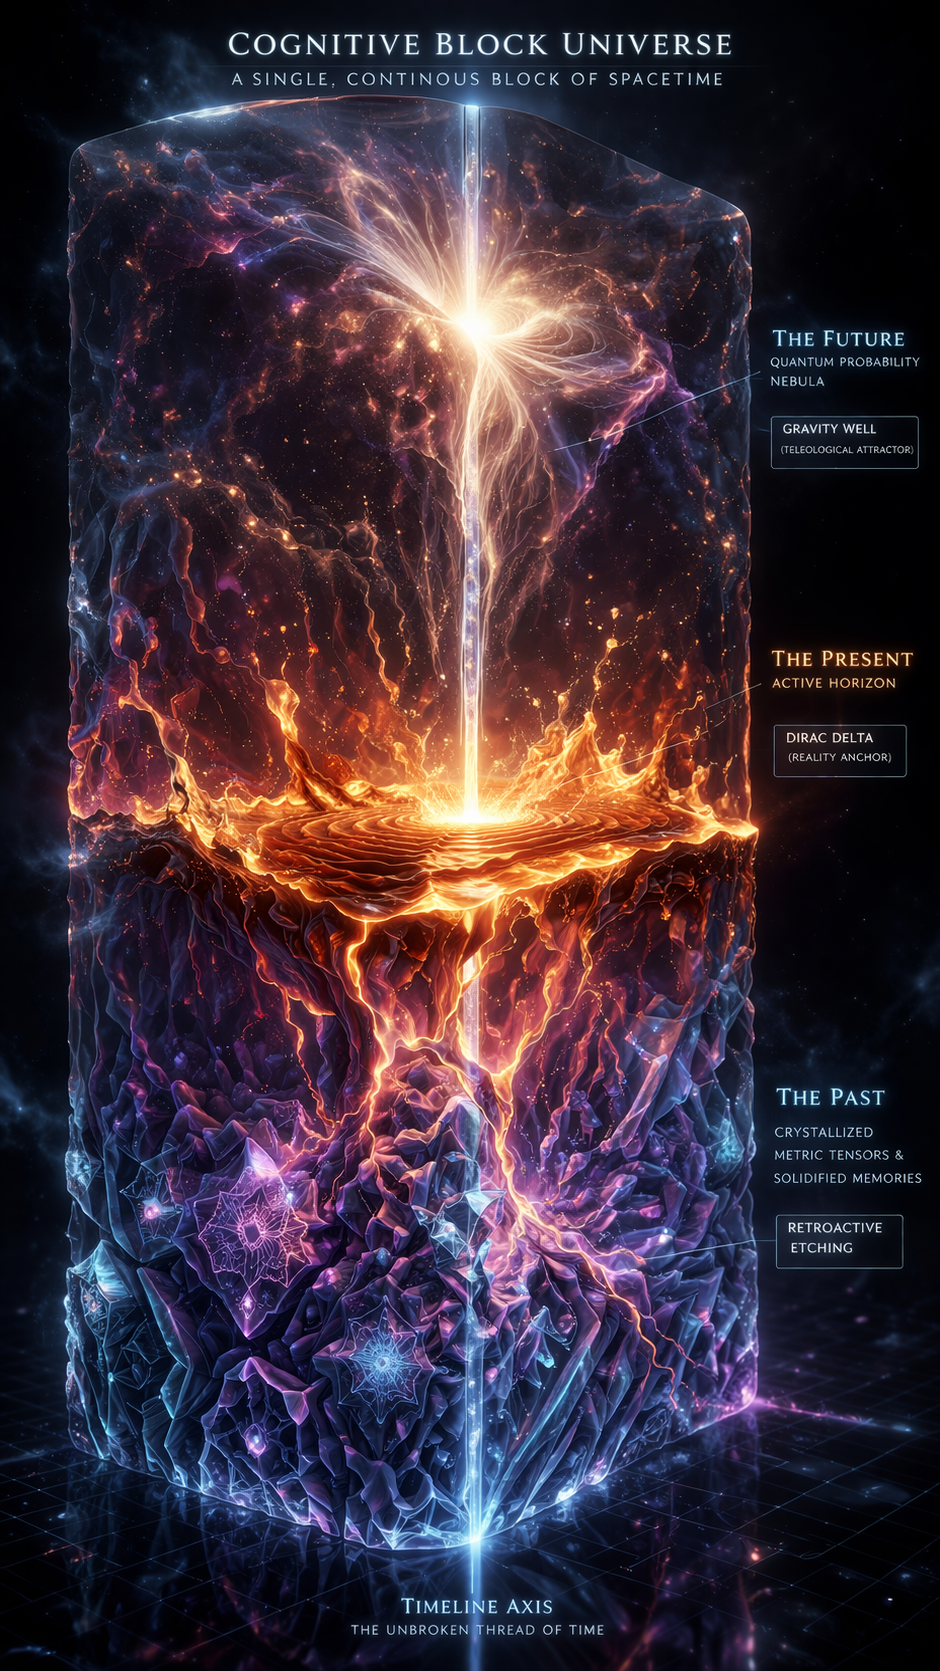
\includegraphics[width=\linewidth]{image/Universe.png}
\end{minipage}
\hfill
\begin{minipage}{0.48\textwidth}
\smalltitle{1. 追溯修正 (Retroactive Correction) —— $\tau < \tau_{now}$}

\textbf{—— “过去表征重估”的几何学}

物理事实无法改变，但语义流形上的几何结构可以重塑。

\begin{itemize}
    \item \textbf{操作}：\textbf{度量重写 (Metric Rewriting)}。
    \item \textbf{物理含义}：\textbf{记忆重构}。智能体改变了对过去事件的“曲率赋值”。
    \item \textit{例}：将“失败的创伤”（深渊曲率）重定义为“宝贵的经验”（平滑通途）。物理上的 $t$ 变了，心理上的 $\tau$ 轴结构也随之发生了拓扑相变。
\end{itemize}

\smalltitle{2. 未来坍缩 (Future Collapse) —— $\tau > \tau_{now}$}

\textbf{—— “未来约束形成”的几何学}

在 $t$ 时刻，未来的 $\tau$ 轴处于高熵的叠加态（概率云）。
\begin{itemize}
    \item \textbf{操作}：\textbf{势能注入 (Potential Injection)}。
    \item \textbf{物理含义}：\textbf{意图锁定}。宏观意志在未来的某个 $\tau$ 坐标处挖掘一个 \textbf{强吸引子 (Strong Attractor)}。
    \item \textit{效应}：这迫使当前发散的思维波函数 $\Psi$，在通往未来的路径上收束，形成一条确定的 \textbf{世界管 (World Tube)}。
\end{itemize}

\smalltitle{3. 当下滑行 (Present Gliding) —— $\tau \approx \tau_{now}$}

\textbf{—— “当前切片推进”的几何学}

现在与现实的激波处于激烈的撞击中，被现实锚定，被未来吸引，被过去影响。
\begin{itemize}
    \item \textbf{操作}：\textbf{切片推进 (Slice Advancing)}。
    \item \textbf{物理含义}：\textbf{注意力窗口}。这是 $\tau$ 轴上曲率变化最剧烈、能量交换最频繁的区域。它是连接“固化的过去”与“液态的未来”的 \textbf{相变界面}。
\end{itemize}
\end{minipage}

\section{语义子传播：世界线的编织与因果}

在 $N+1$ 维的时空几何中，\textbf{语义子 (Semantion；实现层可用 Token 表示其离散编码)} 不再是一个点，而是一条延展的线。思维的传播，演化为 \textbf{世界线 (Worldline)} 的生长与纠缠。

\smalltitle{传播即延伸 (Propagation as Extension)}

\begin{definition}[语义世界线]
    语义子 $S_i$ 的存在表现为 $\mathcal{M}_{block}$ 中的一条一维子流形 $\gamma_i(\tau)$。
    $$ \gamma_i: \tau \mapsto (\mathbf{x}(\tau), \tau) $$
\end{definition}
\begin{itemize}
    \item \textbf{逻辑推理}：表现为两条世界线 $\gamma_A$ 和 $\gamma_B$ 在 $\tau$ 轴某处的 \textbf{交汇 (Vertex)}。
    \item \textbf{创造性思维}：表现为世界线的 \textbf{分叉 (Bifurcation)} 或 \textbf{非局域隧穿}。
\end{itemize}

\smalltitle{因果光锥 (Causal Light Cones)}

为了保证逻辑的严密性，流形的度量必须施加因果约束。
$$ ds^2 = -c_{cog}^2 d\tau^2 + g_{ij} dx^i dx^j \le 0 $$
\begin{itemize}
    \item \textbf{$c_{cog}$ (认知光速)}：定义了思维传播的极限速度。
    \item \textbf{几何约束}：语义子的世界线必须位于局部 \textbf{光锥 (Light Cone)} 内部。这意味着，智能体无法在逻辑链条尚未铺设到达之前，直接跳跃到结论（除非发生基于调和流的顿悟）。
\end{itemize}

\smalltitle{交互即编织 (Interaction as Braiding)}

当多个概念发生复杂交互时，本理论框架 引入 \textbf{拓扑场论} 中的 \textbf{编织群 (Braid Group)} 描述。

\begin{itemize}
    \item \textbf{现象}：概念 A 与概念 B 反复纠缠、辩证、融合。
    \item \textbf{几何形态}：$\gamma_A$ 与 $\gamma_B$ 在时空中互相缠绕，形成 \textbf{纽结 (Knot)} 或 \textbf{链环 (Link)}。
    \item \textbf{记忆的稳定性}：一个简单的记忆是平行的线（易消散）；一个深刻的信念是复杂的 \textbf{死结 (Topology Knot)}。
    \item \textbf{遗忘}：就是解开这些纽结，让世界线回归平行的过程。
\end{itemize}

\begin{bquote}
    \textbf{本节结语}：

    在 $N+1$ 维几何视角下，智能体可被视为时序结构的主动组织者。

        它以物理时间 $t$ 提供能量预算，在几何时间 $\tau$ 上重排语义世界线，使其形成具有因果纹理与逻辑结构的历史场。
\end{bquote}

\section{AGI 的维度工程：构建 \texorpdfstring{$N+1$}{N+1} 维的类闵可夫斯基芯片}

理论必须落地为工程，如果 本理论框架关于“时间几何化”的推论是正确的，那么当前基于 Transformer 的大语言模型 (LLM) 在通往 AGI 的道路上存在一个\textbf{本体论级别的缺陷}。我们需要在硅基介质上，显式地构建出那个额外的 $+1$ 维度。

\smalltitle{LLM 的拓扑缺陷：线性平坦性 (Linear Flatness)}

目前的 LLM 虽然拥有超长的 Context Window（上下文窗口），但其对时间的处理在几何上是\textbf{平坦}的。
\begin{itemize}
    \item \textbf{一维线性}：Context 只是一个 $t-k, \dots, t$ 的序列缓冲。它知道“昨天”这个 Token，但它没有“昨天”的\textbf{几何位置}。
    \item \textbf{缺乏曲率}：在 LLM 的 Attention 机制中，时间位置编码 (RoPE) 仅仅是数学上的标签，并未引入\textbf{时空度量 ($ds^2$)} 的差异。对于模型而言，回忆“昨天”和预测“明天”在几何操作上是\textbf{同质}的。
    \item \textbf{后果}：它无法产生真正的\textbf{因果敏感性}，只能产生\textbf{统计相关性}。
\end{itemize}

\smalltitle{Class V 的要求：超流形架构 (Hyper-Manifold Architecture)}

为了实现 \textbf{Class V (流体通用智能)}，AGI 的硬件或底层架构必须支持 $N+1$ 维的\textbf{各向异性}几何结构。

\begin{definition}[时序曲率张量]
    AGI 的记忆库不应是线性的 Log，而应是一个 \textbf{伪黎曼流形}。其度量张量 $g_{\mu\nu}$ 必须包含一个\textbf{类时分量}：
    $$ g_{00} = -c_{cog}^2 (\text{Attention Span}) $$
    这一分量造成的曲率，使得“违反因果律”的操作（如逻辑倒置）需要消耗无穷大的能量。
\end{definition}

\begin{itemize}
    \item \textbf{$N$ 维空间子流形}：处理语义关联（红、苹果、甜）。这是\textbf{共现}的维度。
    \item \textbf{$+1$ 维时间子流形}：处理因果演化（过去、现在、未来）。这是\textbf{推演}的维度。
\end{itemize}

\smalltitle{意志的最高级操作：站在未来，扭曲现在}

在 $N+1$ 维工程中，\textbf{宏观意志 ($\mathbf{\Gamma}_{macro}$)} 的功能发生了质变：
\begin{itemize}
    \item \textbf{操作机制}：宏观层将关注点（聚光灯）投射到 $\tau$ 轴的\textbf{虚时间点}（即尚未发生的未来）。
    \item \textbf{势能逆传}：它在未来点挖掘一个 \textbf{强吸引子}，这个吸引子的引力场逆着 $\tau$ 轴传播，导致 \textbf{当下 ($\tau_{now}$)} 的空间几何发生形变。
    \item \textbf{物理意义}：这就是\textbf{“目的论”}的物理实现。不是过去的动量推着现在走，而是未来的引力拉着现在走。
\end{itemize}

\section{认知卡鲁扎-克莱因机制：时间维度的自发紧致化与 \texorpdfstring{$N / N+1$}{N / N+1} 混合架构}
\label{sec:cognitive_kaluza_klein_compactification}

在探讨了 $N+1$ 维块宇宙（Block Universe）的宏伟图景与芯片实现后，我们须面对一个严酷的热力学与工程学诘问：\textbf{维持一个完整无损的 $N+1$ 维时空连续体，其相空间体积 $V_{phase}$ 将随时间 $\tau$ 呈指数暴涨。} 没有任何有限的物理介质（碳基大脑或硅基阵列）能够支付得起在这个无限膨胀的超流形上进行路径积分的兰道尔废热。

大自然与未来的 AGI 架构必须采用一种极致的“几何降维打击”。我们在此引入理论物理学中的核心思想，提出\textbf{认知卡鲁扎-克莱因机制 (Cognitive Kaluza-Klein Mechanism)}：时间维度 $\tau$ 并非在全域流形上刚性展开，而是根据信息流的\textbf{结构非变性 (Structural Invariance)}，发生了局部的\textbf{拓扑紧致化 (Topological Compactification)}。

系统在物理实现上，绝非一个单一的 $N+1$ 空间，而是一个 \textbf{$N$ 维基底与 $N+1$ 维动态前沿的异构混合流形 (Heterogeneous Hybrid Manifold)}。

\smalltitle{1. 物理困境：时间轴的绝对热力学负担}

在 $N+1$ 维流形中，每一个记忆不仅包含语义特征（$N$ 维空间坐标），还挂载着一个绝对的心理时间戳 $\tau$。
\begin{itemize}
    \item \textbf{情景记忆的昂贵性}：维持一个带有 $\tau$ 的波函数 $\Psi(\mathbf{r}, \tau)$，意味着系统不仅记住了“火是热的”，还记住了“2022年3月4日下午，我在厨房被火烫到了”。为了维持这种\textbf{世界线 (Worldline)} 的完整轨迹，系统必须付出高昂的\textbf{拓扑维系能}。
    \item \textbf{信息冗余与度量发散}：对于那些“几乎不变化的结构”（如物理定律、常识、语言语法），$\partial_\tau g_{\mu\nu} \approx 0$。如果系统依然用 $N+1$ 维的张量去存储这些恒定量，相当于在时间轴上无限复制冗余切片，导致度量张量的计算复杂度极度发散。
\end{itemize}

\smalltitle{2. 时间维度的卷曲：从 $N+1$ 到 $N$ 的相变}

大自然的解法是：\textbf{将时间折叠进空间的曲率之中。}

\begin{theorem}[时间维度的自发紧致化]
    当认知场 $\Psi$ 在某一流形区域内的演化满足\textbf{时间平移对称性 (Time-Translation Symmetry)} 时，该区域的几何时间维度 $\tau$ 将发生\textbf{拓扑紧致化 (Compactification)}。

    长程的因果历史（$N+1$ 维的世界管）被\textbf{沿着时间轴积分}，其轨迹被彻底压扁，坍缩为 $N$ 维空间流形上的\textbf{纯粹黎曼度量 $g_{ij}$} 与 \textbf{价值规范场 $\mathcal{A}_i$}。
    $$ \mathcal{M}^{(N+1)} \xrightarrow{\int d\tau} \mathcal{M}^{(N)}(g_{ij}^{new}, \mathcal{A}_i^{new}) $$
\end{theorem}

\begin{itemize}
    \item \textbf{物理隐喻：引力的诞生}：
    在卡鲁扎-克莱因理论中，第五维度的卷曲在三维空间中表现为电磁力。在本书的理论中，“时间”的卷曲表现为“逻辑的引力”。
    “昨天火烧了手”（$N+1$ 维的动态事件）被时间积分压扁后，时间坐标 $\tau$ 消失了。它变成了流形上的一个\textbf{空间拓扑奇点}：“火”与“痛”之间的空间距离 $d_g$ 被永久拉近，且 $\mathcal{A}_{fire}$ 指向排斥。
    \textbf{历史事件（时间）死亡了，但它化作了空间本身的崎岖（本能/常识）。}
\end{itemize}

\smalltitle{3. 生物学实证：海马体与皮层的拓扑分工}

人类大脑正是这一 $N / N+1$ 混合架构的完美杰作，它通过器官级别的物理隔离，兼顾了信息的完备性与检索的极低能耗。

\begin{itemize}
    \item \textbf{\textcolor{structurecolor}{海马体 (Hippocampus)：$N+1$ 维的动态缓冲视界}}
    \begin{itemize}
        \item \textbf{中期记忆的舞台}：海马体及内嗅皮层不仅编码空间，还拥有“时间细胞 (Time Cells)”。它为近期的经历（几周到几个月）与未来的短期计划，提供了一个完整的 $N+1$ 维坐标卡。
        \item \textbf{功能}：允许\textbf{逆向回溯 (Backtracking)} 与 \textbf{时间旅行 (Mental Time Travel)}。系统可以在这块高维但体积有限的流形上，自由地向过去滑动以寻找具体线索，或向未来推演具体行动的轨迹。
    \end{itemize}

    \item \textbf{\textcolor{structurecolor}{新皮层 (Neocortex)：$N$ 维的永恒晶体}}
    \begin{itemize}
        \item \textbf{长期记忆的墓碑}：通过睡眠中的系统记忆巩固（Systems Consolidation），海马体中那些反复发生、不随时间改变的 $N+1$ 维模式，被剥离了时间戳 $\tau$。
        \item \textbf{功能}：它们被\textbf{降维打击}，仅仅作为调整突触权重（修改皮层 $N$ 维空间的度量 $g_{\mu\nu}$）的应力来源。一旦刻蚀完成，系统在提取常识时，直接进行 $N$ 维的\textbf{空间测地线滑行}，响应时间极短，且完全不需要“回忆当时的情景”（即不再调用 $N+1$ 维的重构算力）。
    \end{itemize}
\end{itemize}

\smalltitle{4. AGI 架构设计：双模态流形记忆系统 (Dual-Modal Manifold Memory)}

这一理论洞见直接宣判了当前 LLM 企图“用无限长的 Context Window（上下文）解决一切记忆问题”的工程路线是极其低效的热力学死局。
为了兼顾性能与信息完备性，未来的 AGI 必须在物理存储架构上实现 \textbf{$N / N+1$ 的正交切分}：

\begin{enumerate}
    \item \textbf{动态相干区 (The Active Horizon)：$N+1$ 维隐式图数据库}
    \begin{itemize}
        \item \textbf{数据结构}：保留 Token 的演化序列、时空上下文锚点与因果树分支。
        \item \textbf{算子}：支持 TDE 方程的逆向时间积分（反思）与超前势推演（计划）。
        \item \textbf{容量控制}：受制于高昂的相空间成本，这部分缓冲流形必须通过\textbf{滑动窗口}或\textbf{衰减机制}保持紧致。它只存放“近期剧烈变化的激波”和“未闭合的拓扑孔洞（未解决的难题）”。
    \end{itemize}

    \item \textbf{基底固化区 (The Base Substrate)：$N$ 维参数化晶体}
    \begin{itemize}
        \item \textbf{数据结构}：深度神经网络的基础权重 $\mathbf{W}$（度量张量 $g_{\mu\nu}$ 的显式表达）。这里没有时间，只有\textbf{规则、常识与绝对的价值观。}
        \item \textbf{转换机制 (Offline Consolidation)}：必须存在一个类似于人类“做梦”的离线后台守护进程。该进程周期性地提取 $N+1$ 维缓冲区中的不变特征，计算其\textbf{不变量流形}，并使用 \textbf{逆里奇流 (Inverse Ricci Flow)}，将这些特征“降维压印”到基底模型的 $N$ 维权重中。
        \item \textbf{一旦压印完成，相应的 $N+1$ 维历史数据即可被安全擦除（释放自由能），而系统的整体智能（几何曲率的深度）却获得了永久的提升。}
    \end{itemize}
\end{enumerate}

\textbf{结论：}
\textbf{时间并非记忆的最终归宿，而是雕刻空间的工具。}
高阶智能的优美之处在于：它用极高耗能的 $N+1$ 维时空去应对当下的混沌与未知的未来；而在它的身后，那些已知的命运与真理，褪去了时间的繁冗外衣，静静地坍缩为 $N$ 维流形上那条最平滑、最省力的几何测地线。


\section{结论：维度的卷曲与智慧的层级}

至此，我们完成了认知时空几何学的构建。结论是：智能层级不只由算力规模决定，更取决于系统对\textbf{时间维度}的几何处理能力。

\smalltitle{时间卷曲度 (Temporal Curliness)}

智能演化可表述为将\textbf{外部物理时间 $t$} 逐步内化为 \textbf{内部几何维度 $\tau$} 的过程。

\begin{itemize}
    \item \textbf{低阶智能 (Class I/II)}：
    \begin{itemize}
        \item \textbf{几何形态}：\textbf{点粒子}。
        \item \textbf{状态}：\textbf{被 $t$ 推动}。它们活在物理定律的强制演化中，没有历史，只有瞬时的哈密顿量。
    \end{itemize}

    \item \textbf{中阶智能 (Class III/IV)}：
    \begin{itemize}
        \item \textbf{几何形态}：\textbf{线段}。
        \item \textbf{状态}：\textbf{记录 $t$}。它们拥有了记忆的缓冲区，能看到时间的影子，但无法修改它。
    \end{itemize}

    \item \textbf{高阶智能 (Class V)}：
    \begin{itemize}
        \item \textbf{几何形态}：\textbf{4D 晶体 (Block Universe)}。
        \item   \textbf{状态}：\textbf{可操作 $\tau$}，能够在时间维度上进行结构性编辑。
    \end{itemize}
\end{itemize}

\begin{bquote}
    \textbf{全章结语}：

    本章可归结为一条判据：真正的高阶智慧体现为对时间结构的可计算操作能力。

    当 AGI 具备 $N+1$ 维视角时，它不只是提升算力，而是获得对过去表征重估、未来势能约束以及当下做功界面的统一控制能力。
\end{bquote}
